Polymorphism from greek means literally \emph{having several forms}, with forms in the sense of \emph{types}.
In general polymorphic are function names (operators, methods, ...) but also types (with parametric data types, constructors, generics, ...).

\section{Flavors of polymorphism}
Polymorphism can have different flavors, to name a few: ad hoc, bounded, contravariant, covariant, inclusion, invariant, parametric, universal, ...
And some of the related concepts, which are basically different implementations inside the various languages are: coercion, generics, inheritance, macros, overloading, overriding, subtyping, templates, ...

\subsection{Universal and ad hoc}
\begin{itemize}
    \item with ad hoc polymorphism the same function name denotes different algorithms, determined by the actual types.
    So we have actual different implementations, different code written by the user based on the type of the data;
    
    \item with universal polymorphism there is only one algorithm, so a single solution applies to objects of different types.
    So we have the same code which is used for different data types.
\end{itemize}

\subsection{Binding time}
The binding of the function name with the actual code to execute can be:
\begin{itemize}
    \item at compile time: early, static binding (also static dispatching);
    \item linking time;
    \item at execution time: late, dynamic binding (also dynamic dispatch).
\end{itemize}
if the binding spans over different phases the binding time is the last one.
For debugging and performance reason the earlier the better!

\subsection{Classification of polymorphism}
\begin{figure}[H]
    \centering
    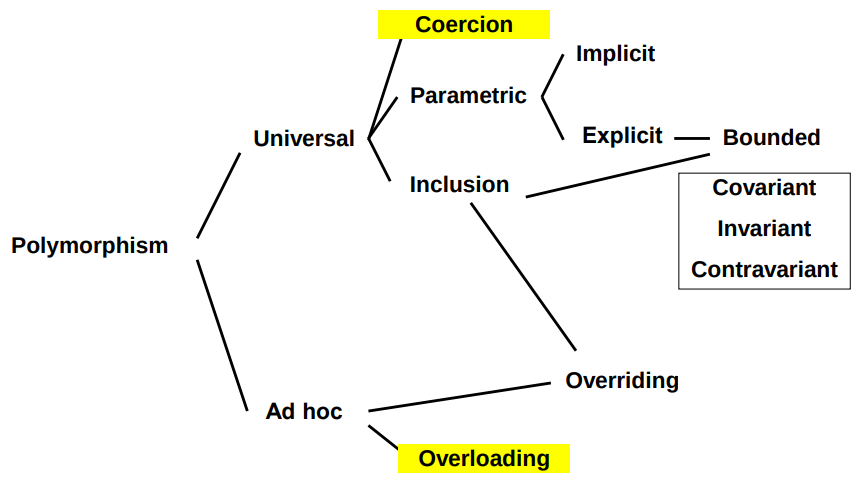
\includegraphics[width=300px]{images/5_Polymorphism/classification.png}
    \caption{Classification of polymorphism}
\end{figure}

\subsection{Ad hoc polymorphism}
\subsubsection{Overloading}
It's a feature present in all languages, at least for built-in arithmetic operators like +, -, * because those operators are defined for different types of data (we have sum between integers and float, sometimes between strings too).
Sometimes it's supported for user defined functions in which you can use the same function name to refer different implementation if differs for the parameter list.

Some languages like C++, Haskell and python even allow the overloading of primitive operators by user defined functions.

The code to execute in case of overloading is determined by the type of the arguments so we can have:
\begin{itemize}
    \item early binding in statically typed languages;
    \item late binding in dynamically typed languages.
\end{itemize}

\subsubsection{Overloading in Haskell}
Haskell introduces type classes (more on this in the haskell chapter) for handling overloading in presence of type inference.
It's a very nice and clean solution and this approach is adopted by Rust too in the concept of \verb|traits|.

\subsection{Universal polymorphism}
\subsubsection{Coercion}
It's the automatic (implicit) conversion of an object to a different type, it's the opposite of casting since it is explicit.
This property can be used to apply the same code to arguments of different type.
In well-designed languages coercion is only possible if there is no loss of information.
It's a degenerate case of polymorphism, not so interesting.

An example:
\begin{verbatim}
double sqrt(double x){ return x*x;}
double d = sqrt(5);     // 5 which is int is converted to double
\end{verbatim}

\subsubsection{Inclusion}
It's also known as subtyping polymorphism or inheritance.
Polymorphism is ensured by substitution principle: an object of a subtype (subclass) can be used in any context where an object of the supertype (superclass) is expected.
Java, C++ (and more) methods/functions with a formal parameter of type \verb|T| accept an actual parameter of type \verb|S| subtype of \verb|T| and methods/virtual functions declared in a class can be invoked on objects of subclasses, unless redefined.

\subsubsection{Overriding}
In Java a method \verb|m| of a class \verb|A| can be redefined in a subclass \verb|B| of \verb|A|:
\begin{verbatim}
class A{
    public void m(){...}
}
class B extends A{
    public void m(){...}
}
...
A a = new B();  // it's legal
a.m()           // will call method m of class B
\end{verbatim}

Overriding introduces ad hoc polymorphism in the universal polymorphism of inheritance.
The resolution of which method to use is done at run-time by the lookup done by the \verb|invokevirtul| opcode of the JVM.

\subsection{Overloading + Overriding in C++ and Java}
Take this example in C++:
\begin{verbatim}
class A{
public:
    virtual void onFoo(){}
    virtual void onFoo(int i){}
};

class B : A{
public:
    virtual void onFoo(int i){}    
};

class C : B{
};

int main(){
    C* c = new C();
    c->onFoo();         // Won't compile!
}
\end{verbatim}
and the almost same implementation in Java:
\begin{verbatim}
class A{
    public void onFoo(){}
    public void onFoo(int i){}
}

class B extends A{
    public void onFoo(int i){}    
};

class C extends B{
};

class D{
    public static void main(String[] args){
        C c = new C();
        c.onFoo();      // Will compile
    }
}
\end{verbatim}

In Java overloading is type-checked by the compiler and override is resolved at run-time by the lookup done by \verb|invokevirtual|.

In C++ instead there is the dynamic method dispatch which means that the compiler adds a v-table (virtual table) to each object from a class that has virtual methods.
The compiler does not see any declaration of \verb|onFoo| in the class \verb|C| so it scans upwards in the class hierarchy checking \verb|B|, it finds the declaration of \verb|void onFoo(int i)| so it stops and tries overload resolution but it fails because of the inconsistencies in the arguments.
So we can say that \verb|onFoo| of \verb|B| hides the one from the superclass.
A solution in this case is to add:
\begin{verbatim}
using A::onFoo;
\end{verbatim}
in the class \verb|B|.

\section{Parametric polymorphism}
The parametric polymorphism is also called generic programming and we will see it in two different shapes:
\begin{itemize}
    \item C++ \emph{templates}: which exists since 1990 and is built around function and class templates with type almost treated as variables.
    Each concrete instantiation produces a copy of the generic code, specialized for that type, this process is called \emph{monomorphization};
    
    \item Java \emph{generics}: which exists since java 1.5 (Java 5) from 2004 and is buit around generic methods and classes, here too almost treating types as variables.
    Those components are strongly type checked by the compiler and exploits \emph{type erasure} for which the type of the variables is \verb|Object| (not completely true) at run-time.
\end{itemize}

\subsection{C++ Generics}
\subsubsection{Polymorphism with macros}
For simple case macros can be used to implement polymorphism:
\begin{verbatim}
#define SQRT(T) T sqrt(T x) { return x*x; }
SQRT(int);      // will define sqrt function for int
SQRT(double);   // will define sqrt function for double
\end{verbatim}
macros are executed by the preprocessor (which basically copy-paste the macro expansion and blindly substitute the placeholder with the specified value without any kind of check) while templates by the compiler.
Macro expansion is visible compiling with the option \verb|-E|.
By the way since macros is just grammatic copy-paste it has a lot of limitations for example it copies the side effects and doesn't allow recursion:
\begin{verbatim}
#define sqr(x) ((x) * (x))
int a = 2;
int aa = sqr(a++);
// will become ((a++) * (a++))


#define fact(n) (n==0) ? 1 : fact(n-1) * n
// after substitution compilation will fail because
// function fact is not defined
\end{verbatim}

\subsubsection{C++ templates}
Function templates in C++ supports parametric polymorphism, type parameters can be of every type, both class and primitive types (unlike Java generics which only supports classes).
An example of polymorphic function is:
\begin{verbatim}
template <class T>  // or <typename T>
T sqrt(T x){
    return x*x;
}
\end{verbatim}
During compilation and linking it is automatically generated a version for each parameter type used by the program.
Parameter types are inferred or indicated explicitly (sometime necessary in the case of ambiguity).
Of course it works for user-defined types as well (in the case of sqrt function the type must define the operator *, though).

Sometimes it is difficult for the compiler to inference the type on its own:
\begin{verbatim}
template <class T>
T max(T a, T b){
    return (a>b) ? a : b;
}
...
int i = 5, j = 6;
long m = 5;
getMax(i, j);   // will produce getMax<int>
getMax(i, m);   // won't work because can produce both
                // getMax<int> coercing long to int
                // getMax<long> coercing int to long
...
\end{verbatim}
in the case of ambiguity you need to specify the types you are working with, so instead of the second call you should use \verb|getMax<int>(i,m)| (or decouple the two arguments creating a template with two parameter type).

Moreover templates can be used with expressions as parameters if the value of the expression can be determined at compile-time (basically a constant expression):
\begin{verbatim}
template <class T, int N>
T fixed_multiply(T val){
    return val*N;
}
...
fixed_multiply<int, 2>(10);
fixed_multiply<int, 2+3>(10);
...
\end{verbatim}

Templates can also be used in specialization defining a template with the same name and more specific parameter (which leads to partial specialization) or no parameter at all (full specialization).
This can be seen as a kind of override because the compiler can choose the most specific applicable template and indeed we can use better implementation for specific kind of types:
\begin{verbatim}
template <typename T> class Set{
    // Primary template
};

template <typename T> class Set<T*>{
    // Partial specialization
};

template <> class Set<char>{
    // Full specialization
};
\end{verbatim}

Some more insights on C++ templates:
\begin{itemize}
    \item compilation happen on demand so the code is not compiled until an instantiation is required;
    \item the instantiation happens during compile time so it is \emph{static binding}:
    \begin{itemize}
        \item compiler chooses template that is best match based on specialization of the matching templates;
        \item then the template instance is create tacking the template and substituting the types.
        This phase can also be done after parsing so can be language-aware;
        \item in the end there is the overloading resolution, in particular the compilation will fail if some operators are not defined for the type instanced.
    \end{itemize}
    \item compiler needs declaration and definition to instantiate a new template so, instead of splitting those in two files (header file and actual implementation) it is in use to put both inside the same file;
    \item C++ templates are invariant so if $S <: T$ ($S$ is subtype of $T$), then $X<S>$ has no relationship with $X<T>$.
\end{itemize}

\subsubsection{Template metaprogramming}
Templates can be used by a compiler to generate temporary code which then will be merged to the rest of the source and then compiled.
It is Turing complete but can only work with constant expression, it has no mutable variables and is not really supported by IDE's, compilers and other tools.
For example:
\begin{verbatim}
#include <iostream>
int triangular(int n) {
    return (n == 1)? 1 : triangular(n-1) + n;
}
int main () {
    int result = triangular(20);
    std::cout << result << '\n';
}
\end{verbatim}
using metaprogramming we can force the calculation of values of \verb|triangular| at compile time:
\begin{verbatim}
#include <iostream>
template <int t>
constexpr int triangular() {
    return triangular<t - 1>() + t;
}
template <>
constexpr int triangular<1>() {
    return 1;
}
int main () {
    int result = triangular<20>();
    std::cout << result << '\n';
}
\end{verbatim}
the keyword \verb|constexpr| forces the compiler to evaluate the expression.


\subsection{Java Generics}
Java generics implements explicit parametric polymorphism.
It enables classes, interfaces and methods to have type parameters that can be used arbitrarily in the definition.
They can be instantiated by providing arbitrary type arguments.
Java generics have some issues that we will discuss.
Generic example:
\begin{verbatim}
interface List<R>{
    boolean add(E n);
    E get(int index);
}

// then we can have
// List<Integer>
// List<Number>
// List<String>
// Lst<List<String>>
\end{verbatim}

\subsubsection{Generic methods}
Methods can use type parameters of the class if any or can introduce their own one.
For example:
\begin{verbatim}
public static <T> T getFirst<List<T> list){...}
\end{verbatim}
When invoking the generic method you must instantiate all type parameters, explicitly or implicitly (compiler will use some kind of type inference).

\subsubsection{Bounded type parameters}
We can restrict the types that a generic can use inserting some constraint:
\begin{verbatim}
// This class accepts only types that extends Number
// so only subtype of Number
class NumList<E extends Number>{
    void m(E arg){
        arg.intValue();
    }
}
\end{verbatim}

We have some type bounds:
\begin{itemize}
    \item \verb|<T extends Type>|: it's an upper bound, we specify that the parameter type must be sub-type of \verb|Type|;

    \item \verb|<T extends ClassA & InterfaceB & InterfaceC & ...>|: it's a multiple upper bound, we specify both class and some interface that the type \verb|T| must implement;

    \item \verb|<T super Type>|: it's a lower bound, we specify that the parameter type must be a super type of \verb|Type| (\verb|Type| is ok too). 
\end{itemize}

Those type bounds guarantee that the type argument supports the operations used in the method body.
Differently from C++ those bounds ensures that the overloading of the operators will succeed instead of failing after the substitution.

For example: let's implement an algorithm which finds the biggest element in a collection, we need to compare elements so the type parameter must ensure that the \verb|Comparable| interface is defined so we will use as type parameter the bound \verb|<T extends Comparable<T>>|.

\subsubsection{Java rules for generics}
The introduction of Generics in Java has been pervasive because all the APIs were generalized and the backwards compatibility has been obtained through \emph{type erasure}.
Of course there are still some features of the language that are not compatible with the generics, in particular we will discuss:
\begin{itemize}
    \item inheritance;
    \item arrays.
\end{itemize}

\subsubsection{Generics and sub-typing}
Since \verb|Integer| is sub-type of \verb|Number| we would think that \verb|List<Integer>| must be a sub-type of \verb|List<Number>| but that's not the case.

The Java rules are in fact:
\begin{itemize}
    \item given two concrete types \verb|A| and \verb|B|, then \verb|myClass<A>| has no relationship with \verb|myClass<B>|, even if the first one have some kind of relation.
    So sub-typing in java is \emph{invariant} for generic classes;

    \item the common parent of \verb|myClass<A>| and \verb|myClass<B>| is \verb|myClass<?>| (\verb|?| is a wildcard we will see later);

    \item but if \verb|A| is sub-type of \verb|B| and they are generic classes then \verb|A<x>| is sub-type of \verb|B<x>|.
\end{itemize}

\subsubsection{Two cents on covariance and contravariance}
Covariance: enables you to use a more derived type than originally specified.
Contravariance: enables you to use a more generic (less derived) type than originally specified.

More formally we can say that: if $A <: B$ and $F$ is an operator which takes a type and return another one, then:
\begin{itemize}
    \item if $F(A) <: F(B)$ then $F$ is covariant;
    \item if $F(B) <: F(A)$ then $F$ is contravariant;
    \item if $F(A)$ has no relationship with $F(B)$ then $F$ is invariant.
\end{itemize}

Let's take this code:
\begin{verbatim}
RoList<Integer> lisInt = new …;
RoList<Number> lisNum = new …;
lisNum = lisInt;
Number n = lisNum.get(0); 
\end{verbatim}
since we are just reading from the list it could be correct to get element of type \verb|Integer| into type \verb|Number|, so a \emph{covariant} notion of sub-type would be safe as it is generally for read-only type.

Now let's take this code instead:
\begin{verbatim}
WoList<Integer> lisInt = new …;
WoList<Number> lisNum = new …;
lisInt = lisNum;
lisInt.add(new Integer(…));
\end{verbatim}
we are only writing elements of type \verb|Integer| so a \emph{contravariant} notation of sub-type would be safe as it is generally for write-only type.

Though in the general case neither of both interpretation could be correct since we read and write to structures so Java language decided to block both notations giving type mismatch error.

\subsubsection{Arrays and generics}
Arrays are built-in containers so let's take \verb|Type1| as sub-type of \verb|Type2| then \verb|Type1[]| is a sub-type of \verb|Type2[]| so the arrays in Java are covariant.
This property has been fixed in the rule before the introduction of the generics because otherwise:
\begin{verbatim}
void sort(Object[] o){...}
\end{verbatim}
could not work without creating a different sort implementation for each subtype of Object, but since sorting does not inserts new objects in the array it can't cause errors if used covariantly.

In general this property could cause some problems:
\begin{verbatim}
// Apple and Strawberry both extends Fruit
Apple[] apples = new Apple[1];
Fruit[] fruits = apples;        // ok for covariance
fruits[0] = new Strawberry();   // will compile but at
                                // runtime ArrayStoreException
\end{verbatim}

To solve this problem Java add a run-time check on every array update, since the dynamic type of an array is known at run-time the JVM knows that the array bound for \verb|fruit| is \verb|Apple[]| (\verb|LApple|) so it can check during update for type mismatch and throws \verb|ArrayStoreException|.

\subsubsection{Generics, array of generics and type erasure}
All type parameters of generic types are transformed to \verb|Object| or to the first bound after compilation in order to gain backward compatibility and to give the same type to all the instances of the same generic type:
\begin{verbatim}
List<String> l1 = new ArrayList<String>();
List<Integer> l2 = new ArrayList<String>();
l1.getClass() == l2.getClass();     // true
\end{verbatim}

Since every update in java array must include a run-time check and the generic types are not present at the run-time because of the type erasure then array of generics are not supported in Java.
In fact they would cause type errors not detectable at run-time since each generic would be the same type despite their actual parameter types.

\subsubsection{Wildcards}
Invariance of generic classes is restrictive but can be relaxed using wildcards.
Let's suppose:
\begin{verbatim}
interface Set<E>{
    void addAll(???E);
}
\end{verbatim}
what could be a type to use to define the parameter for the method?
We would like to be able to add \verb|Set<E>| but also all the other collections, so we could use \verb|Collection<E>| but even the sub-types of \verb|E| could be inserted, so the actual answer is \verb|Collection<? extends E>|.

Basically \verb|?| is an anonymous variable, can be used when the type is used exactly once and the name of the type is unknown.
They are used for use-site variance (not declaration-site variance).

Some other syntaxes are:
\begin{itemize}
    \item \verb|? extends T|: denotes every sub-type of \verb|T|.
    Used when we want to get values from the producer, in order to support covariance;

    \item \verb|?|: shorthand for \verb|? extends Object|;

    \item \verb|? super T|: denotes every super-type of \verb|T|.
    Used when we want to insert values in the consumer, in order to support contravariance.
\end{itemize}
Whenever we want to both produce and consume we don't use wildcard.
The principle is \emph{PECS}: Producer Extends, Consumer Super.

\subsubsection{Limitations of Java Generics}
Limitations are there mostly because of the type erasure:
\begin{itemize}
    \item we cannot instantiate generic types with primitive types;
    \item cannot create instances of type parameters;
    \item cannot declare static fields whose types are type parameters;
    \item cannot use casts or \verb|instanceof| with parameterized types;
    \item cannot create arrays of parameterized types;
    \item cannot create, catch or throw objects of parameterized types;
    \item cannot overload a method where the formal parameter types of each overload erase to the same raw type:
\begin{verbatim}
public class Example{
    public void print(Set<String> s){...}
    public void print(Set<Integer> i){...}
}
// won't compile
\end{verbatim}
\end{itemize}


\subsection{Generics and sub-types in C\#}
In C\# the type parameter of a generic class can be annotated \verb|out| for covariant, \verb|in| for contravariant, otherwise it is invariant.
For example \verb|IEnumerator| is covariant because the only method returns the data so it is read-only while \verb|IComparable| is contravariant because the only method accepts a value of type specified, so in some sense is write-only.


\subsection{Covariance and Contravariance in Scala}
Scala too supports annotations to specify covariance and contravariance with \verb|-| and \verb|+| for type parameters:
\begin{verbatim}
class VendingMachine[+A]{...}

class GarbageCan[-A]{...}

trait Function1[-T, +R] extends AnyRef
{ def apply(v1:T):R }
\end{verbatim}





